%%%%%%%%%%%%%%%%%%%%%%%%%%% asme2e.tex %%%%%%%%%%%%%%%%%%%%%%%%%%%%%%%
% Template for producing TSFP-format articles using LaTeX
% Based on the asme2e template (http://iel.ucdavis.edu/code/ASME/)
% Modified: 30 January 2011 for TSFP7 by C. Vanderwel
% Modified: 11 February 2013 for TSFP8 by R. Manceau
% Modified: 05 May 2014 for TSFP9&10 by K. Chauhan (kapil.chauhan@sydney.edu.au)
% Modified: 15 May 2018 for TSFP11 by C. Vanderwel (c.m.vanderwel@soton.ac.uk)
% Modified: 16 December 2024, 04 July 2025 for TSFP14 by K. V. Wilhelm (wilhelm@fdy.tu-darmstadt.de)
%%%%%%%%%%%%%%%%%%%%%%%%%%%%%%%%%%%%%%%%%%%%%%%%%%%%%%%%%%%%%%%%%%%%%%

%%%%%%%%%%%%%%%%%%%%%%%%%%%%%%%%%%%%%%%%%%%%%%
% To generate a pdf, compile either with pdflatex
% or with latex and
% dvips tsfp_template -Ppdf -t a4 -o
% followed by
% ps2pdf tsfp_template.ps
% (avoid using dvipdf that does not preserve the page layout on some systems)
%%%%%%%%%%%%%%%%%%%%%%%%%%%%%%%%%%%%%%%%%%%%%%

%%% use twocolumn and 10pt options with the tsfp format
\documentclass[twocolumn,10pt]{tsfp}
\usepackage{flushend}
\usepackage{graphicx}
\usepackage[authoryear,round]{natbib}
\usepackage{fancyhdr}
\usepackage{amsmath}
\usepackage{subcaption}


\pagestyle{fancy}
\fancyhf{}
\renewcommand{\headrulewidth}{0pt}
\chead{14th International Symposium on Turbulence and Shear Flow Phenomena (TSFP14) \\ Heidelberg, Germany, July 28--31, 2026}
\cfoot{\thepage}


\title{Transition mechanisms in laminar boundary layers over surface gaps}

%%%% In case you need to slightly adapt the horizontal spacing between authors (for more than 3 authors) uncomment the following command
%%%% and if necessary modify the factor
%\renewcommand{\expauthors}{1.1}

%%% first author
\author{Víctor Ballester Ribó
\affiliation{
    Department of Aeronautics\\
    Imperial College London\\
    London, UK\\
v.ballester-ribo24@ic.ac.uk
}	
}

%%% second author
%%% remove the following entry for single author papers
%%% add more entries for additional authors
\author{Jeffrey D. Crouch
      \affiliation{\\
    The Boeing Company\\
    Seattle, USA\\
    jeffrey.d.crouch@boeing.com
}
}


%%% third author
%%% remove the following entry for single author papers
%%% add more entries for additional authors
\author{Yongyun Hwang
		  \affiliation{Department of Aeronautics\\
	Imperial College London\\
	London, UK\\
	y.hwang@imperial.ac.uk
	}
}

%%% fourth author
%%% remove the following entry for single author papers
%%% add more entries for additional authors
\author{Spencer J. Sherwin
		  \affiliation{Department of Aeronautics\\
	Imperial College London\\
	London, UK\\
	s.sherwin@imperial.ac.uk
	}
}

\begin{document}
\maketitle   %Print title matter
\thispagestyle{fancy}

% Set the font to 9pt.
\fontsize{9}{11}\selectfont

%%%%%%%%%%%%%%%%%%%%%%%%%%%%%%%%%%%%%%%%%%%%%%%%%%%%%%%%%%%%%%%%%%%%%%

%%%%%%%%%%%%%%%%%%%%%%%%%%%%%%%%%%%%%%%%%%%%%%%%%%%%%%%%%%%%%%%%%%%%%%
\section*{ABSTRACT}
This study investigates the transition of flow over surface gaps in two-dimensional incompressible laminar boundary layers. Using a high-fidelity spectral/$hp$ element solver, we solve the incompressible Navier–Stokes equations to examine how variations in gap geometry influence boundary-layer stability. By tracking the downstream growth of Tollmien–Schlichting waves within the classical $e^n$ framework, we quantify how gaps modify the amplification of primary instabilities relative to smooth-wall configurations. Nonlinear simulations further reveal a sequence of bifurcations as the gap width increases, including quasi-periodic oscillations and signatures of chaotic dynamics for certain geometries. Numerical predictions are validated against experimental data, showing strong agreement. These findings provide new physical insight into the instability mechanisms triggered by surface gaps, extending beyond prior studies that primarily characterized TS-wave amplification.

% demonstrates that both gap width and depth critically affect flow stability, with direct implications for surface design in next-generation low-drag aircraft. The study concludes with proposed extensions to compressible flows and three-dimensional configurations to better capture transition phenomena in more realistic flight conditions.
\section*{INTRODUCTION}
Aircraft wings are not perfectly smooth; instead, they often exhibit small surface discontinuities, commonly referred to as gaps. Although these discontinuities are typically small in scale, they can significantly affect the development of the boundary layer, particularly its transition from laminar to turbulent flow. 

Several studies have investigated the effect of surface gaps or cavities on boundary-layer transition.

ONERA (\emph{Office National d'Études et de Recherches Aérospatiales}) has recently conducted several experimental, numerical, and theoretical studies on the influence of surface gaps on boundary-layer behavior. The work by~\cite{beguetONERA} provides a comprehensive summary of these investigations. Gap geometry is characterized in terms of $w/\delta^*$ and $d/\delta^*$, where $w$ and $d$ denote the width and depth of the gap, respectively, and $\delta^*$ is the displacement thickness of the boundary layer. Their study classifies vortex structures forming within the gap as functions of $w$ and $d$, focusing on gaps with aspect ratios $d/w \in [0.2, 0.7]$. Regarding the $n$-factor, the authors adopt the notation $\Delta n = n - n_0$, where $n$ denotes the $n$-factor for the gapped configuration and $n_0$ corresponds to the smooth flat-plate case. They report two primary effects: first, surface gaps amplify pre-existing Tollmien--Schlichting (TS) waves, as evidenced by increases in $\Delta n$ downstream of the gap; second, the gaps generate localized instabilities, leading to a peak in $\Delta n$ at the gap location. All these results were obtained under incompressible flow conditions.

\cite{zahnRist} performed numerical simulations to examine the influence of deep gaps ($d/w \geq 5$) in compressible boundary-layer flows at a Mach number of $M = 0.6$. They observed non-monotonic behavior of $\Delta n$ as a function of gap depth, with values ranging from 0 to 0.5. In addition to this work, the review by~\cite{dynandcontrol} summarizes different methods methods for analyzing and controlling cavity flows in  high-Reynolds-number compressible regimes. Particular emphasis is placed on the coupling between shear-layer instabilities, acoustic feedback, and recirculating vortices inside the cavity, which are relevant for deep gaps.

One of the most recent and detailed investigations was conducted by~\cite{jeffGaps}, who extensively analyzed the amplification of TS waves over gaps with varying widths and depths. They found that for shallow gaps ($d/w < 0.017$), the $\Delta n$ factor depends primarily on the gap depth $d$ and is independent of the width $w$. Conversely, for deep gaps ($d/w > 0.028$), the $\Delta n$ is governed by the gap width. When both $d$ and $w$ are sufficiently large, the TS-wave-induced transition is bypassed entirely, and the flow transitions to turbulence near the downstream edge of the gap. Their results also suggest that the behavior of shallow gaps resembles that of isolated backward-facing steps.

In this work, we conduct a systematic study of surface gaps by varying both gap width and depth in order to clarify the underlying physics and instability mechanisms across different configurations. We investigate the influence of surface gaps on boundary-layer transition using a combination of Direct Numerical Simulations and Linear Stability Theory in the incompressible regime. As a validation step, we aim to reproduce and interpret the experimental findings of~\cite{jeffGaps}. Future work will focus on explaining the physical mechanisms of transition in long, shallow gaps ($w/d \sim 0.015$) and narrow, deep gaps ($d/w \sim 0.25$).

The transition modelling employed in this work is based on the classical $e^n$ approach, in which linear perturbations (typically TS waves) are tracked as they amplify downstream within the laminar boundary layer according to $A(x) = A(x_0) \mathrm{e}^{n(x)}$. Transition is assumed to occur once the disturbance growth reaches a critical $n$ value. To quantify the influence of the gap, we introduce the $\Delta n$ factor, defined as the difference between the $n$ values obtained for the gapped and smooth configurations. 

From a computational standpoint, we solve the incompressible Navier--Stokes equations using the spectral/$hp$ element method, which combines the geometric flexibility of finite elements with the accuracy of spectral methods. All simulations are performed using the open-source \texttt{Nektar++} framework.

\section*{NONLINEAR SIMULATIONS RESULTS}elucidating
We performed a series of 2D incompressible direct numerical simulations of boundary-layer flow over surface gaps of varying geometries. Gaps are fully characterized by their width $w$ and depth $d$. The range of parameters considered is $w/\delta^* \in [0,130]$ and $d/\delta^* \in [0,4]$, where $\delta^*$ is the displacement thickness of the boundary layer at the gap location. All results are obtained for a Reynolds number of $\mathrm{Re}_{\delta^*} = u_\infty \delta^*/\nu = 1000$, where $u_\infty$ denotes the free-stream velocity and $\nu$ the kinematic viscosity. The results are summarized in Figure~\ref{fig:stability}.

The configurations illustrated in Figure~\ref{fig:stableSS} correspond to $(w/\delta^*, d/\delta^*) \in \{(15,4), (30,1.5), (60,1)\}$. We observe that for deep gaps, a prominent recirculating region forms near the downstream edge of the cavity. In contrast, shallow gaps do not accommodate such structures; the flow instead enters and exits the cavity more smoothly, exhibiting a weak recirculation zone near the upstream edge, resembling the one observed in backward-facing step flows.

For fixed gap depth, increasing the width induces a sequence of bifurcations. When the width surpasses a critical threshold that depends on the depth, the flow becomes unstable. For deep gaps ($d/\delta^* \in [2.5, 4]$), this transition occurs abruptly, while shallower configurations ($d/\delta^* \in [1.5, 2.25]$) exhibit a linearly unstable regime. In this latter region, a Hopf bifurcation emerges, introducing one unstable frequency. A second frequency appears soon after, producing quasi-periodic dynamics on a two-dimensional attracting torus. Spatially, this corresponds to an unstable global mode whose amplitude is concentrated near the downstream edge of the gap. As analyzed by~\cite{GharibRoshko1987} this region correspond to low cavity drag gaps. As the width increases further, the attracting torus becomes increasingly distorted. Additional frequencies become less stable, leading ultimately to a chaotic regime.

\section*{LINEAR SIMULATIONS RESULTS}
Based on the DNS results, we identify several steady base flows $\mathbf{U}$ that serve as a foundation for linear stability analysis. To excite TS waves, a divergence-free perturbation is introduced at the upstream region of the boundary layer to both horizontal and vertical components of the disturbance field $\mathbf{u}'$. This perturbation is modeled as white Gaussian noise. To compare with the experimental data of~\cite{jeffGaps}, we compute the streamwise average of the difference between the $n$-factor of each gapped configuration and that of the flat-plate reference case. This difference is denoted by $\Delta n$. Interpolation is performed inside the convex hull of these points fitting a Gaussian Process Regressor with a radial basis function kernel. The contour plot in Figure~\ref{fig:nfactor} presents a comparison between our simulated $\Delta n$ contours (blue lines) and the fitted experimental results (magenta lines) reported by \cite{jeffGaps} for $\Delta n=1,2,3,4$.

Overall, the comparison with experimental data shows very good agreement, which suggests that the instabilities leading to the amplification of TS waves are two-dimensional in nature. In particular, we correctly capture both asymptotic regimes: the vertical trend at narrow gaps and the horizontal trend at shallow gaps.

\section*{FUTURE WORK}
Future work will significantly extend the present incompressible analysis in three main directions. 

First, the computational framework will be extended to compressible flows to investigate how Mach number influences gap-induced transition. This extension is crucial as compressibility significantly alters the base flow profile and the mechanism by which pressure disturbances are transmitted, potentially introducing new instability modes that are not present in the incompressible regime. The primary goal is to establish a correlation between the $\Delta n$ factor and the Mach number for a fixed gap geometry.

Another important direction involves systematically studying the asymptotic behaviors in two distinct limiting regimes of gap geometry to isolate the dominant physical mechanisms driving transition. These regimes are shallow gaps with large widths, where the gap resembles a backward-facing step, and thus, the $\Delta n$ factor is expected to be a function of the gap depth only; and shorter gaps, where the gap is deep and narrow, and the $\Delta n$ factor is primarily influenced by the gap width (see Figure~\ref{fig:nfactor}).

Finally, the computational mesh will be extruded into three dimensions to account for spanwise effects and three-dimensional instabilities. This step is essential for assessing how secondary instabilities and crossflow-like mechanisms interact with gap-induced disturbances.

%%%%%%%%%%%%%%%%%%%%%%%%%%%%%%%%%%%%%%%%%%%%%%%%%%%%%%%%%%%%%%%%%%%%%%
\bibliographystyle{tsfp}
\bibliography{tsfp}
%%%%%%%%%%%%%%%%%%%%%%%%%%%%%%%%%%%%%%%%%%%%%%%%%%%%%%%%%%%%%%%%%%%%%%
%%%% FIGURES %%%%%
\newpage

% \begin{figure*}
% 	\centering
% 	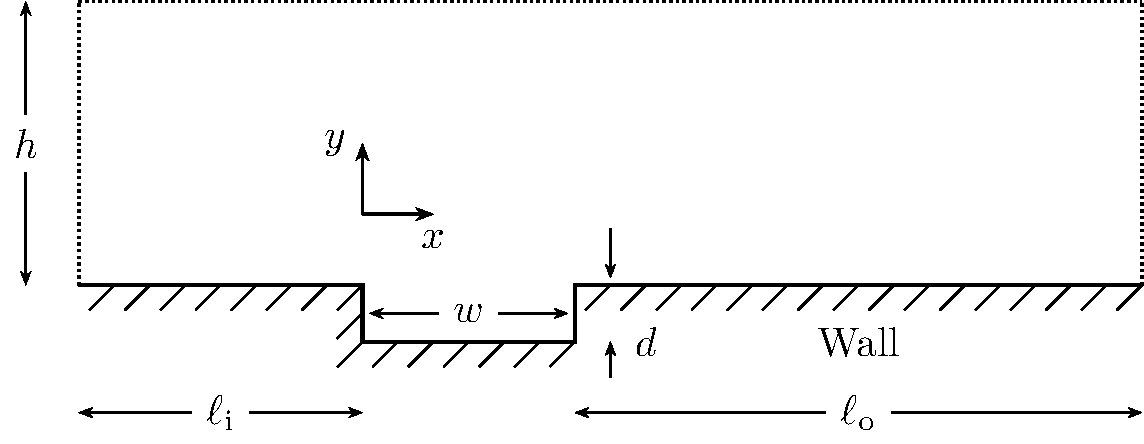
\includegraphics[width=3in]{../../Images/domain.pdf}
% 	\caption{Schematic of the numerical domain used for the 2D incompressible simulations. The gap is characterized by its width $w$ and depth $d$. The boundary layer thickness at the gap location is denoted by $\delta^*$.}
% 	\label{fig:domain}
% \end{figure*}
\begin{figure*}
	\centering
	\includegraphics[width=3.5in]{../../Images/incNS2dStabilityCurve.pdf}
	\caption{Stability diagram showing the dynamical regimes for different gap configurations at $\mathrm{Re}_{\delta^*} =1000$. Gap width $w$ is shown along the horizontal axis and gap depth $d$ along the vertical axis. Blue circles denote steady solutions (equilibria), orange squares represent time-periodic attractors, and black triangles indicate chaotic or turbulent states. The dotted orange line indicate a qualitative boundary for the first Hopf bifurcation while the dashed black line indicate the transition to chaos.}
	\label{fig:stability}
\end{figure*}

\begin{figure*}[ht]
	\centering
	\begin{subfigure}[b]{0.33\textwidth}
		\centering
		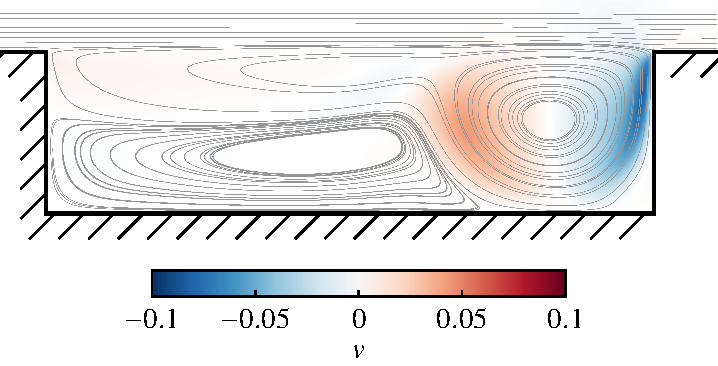
\includegraphics[width=\textwidth]{../../Images/gapd4_w15.pdf}
		\caption{Gap with $w=15\delta^*$ and $d=4\delta^*$.}
		\label{fig:gapd4w15}
	\end{subfigure}\hfill
	\begin{subfigure}[b]{0.33\textwidth}
		\centering
		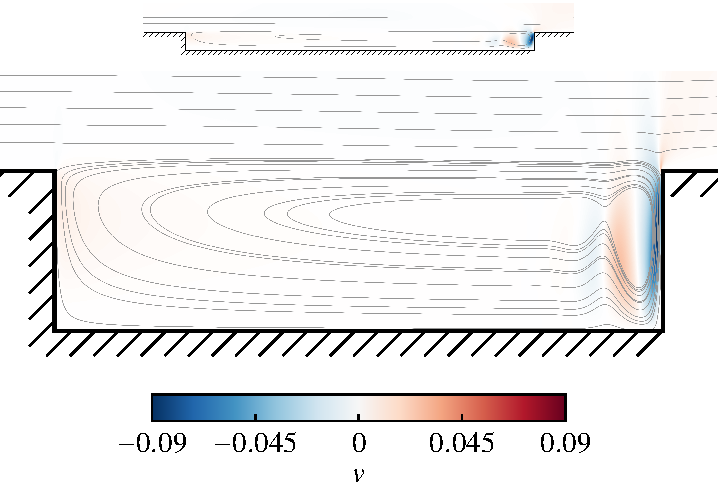
\includegraphics[width=\textwidth]{../../Images/gapd1.5_w30.pdf}
		\caption{Gap with $w=30\delta^*$ and $d=1.5\delta^*$.}
		\label{fig:gapd15w30}
	\end{subfigure}
	\begin{subfigure}[b]{0.33\textwidth}
		\centering
		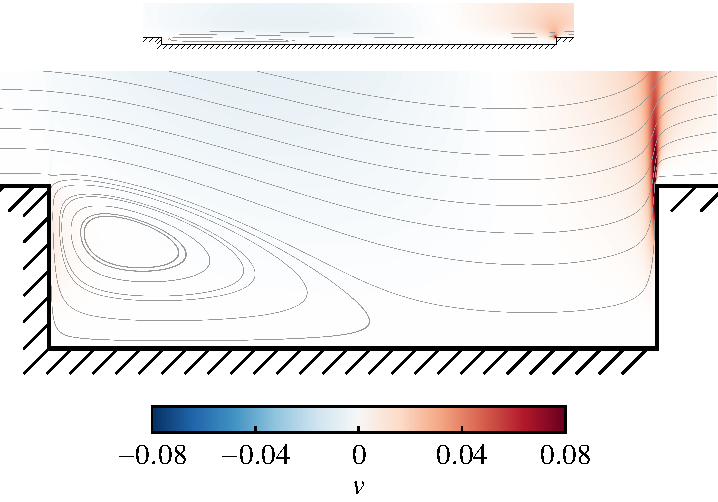
\includegraphics[width=\textwidth]{../../Images/gapd1_w60.pdf}
		\caption{Gap with $w=60\delta^*$ and $d=1\delta^*$.}
		\label{fig:gapd1w60}
	\end{subfigure}
	\caption{Steady-state flow over three different gap configurations. Wall-normal velocity contours and streamlines are shown in each case. All geometries are rescaled to match the size of the first configuration ($w/d = 15/4$) for visual comparison. The original, unscaled geometries are displayed above the last two cases for reference.}
	\label{fig:stableSS}
\end{figure*}

\begin{figure*}
	\centering
	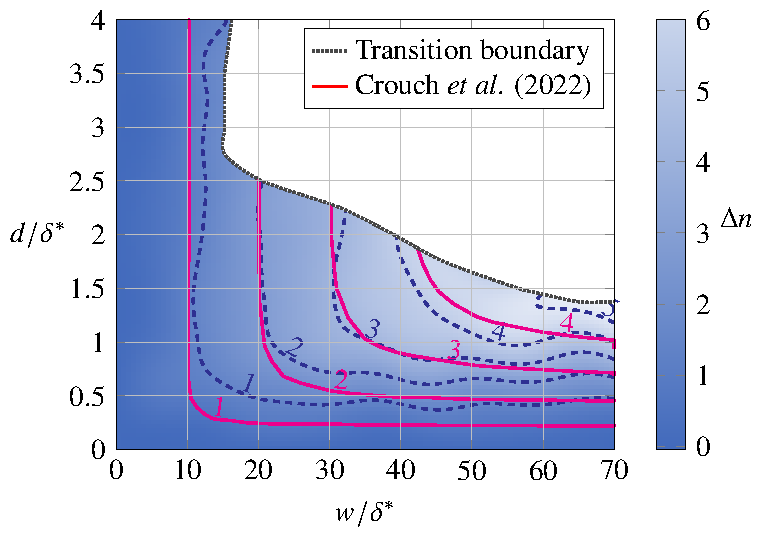
\includegraphics[width=4in]{../../Images/nfactor_countour.pdf}
	\caption{Contour plot of $\Delta n$ factors on the stable side of the parameter grid $(w/{\delta^*},d/{\delta^*})\in[0,70]\times[0,4]$. Magenta contours show experimental level lines from~\cite{jeffGaps} for levels 1, 2, 3, and 4.}
	\label{fig:nfactor}
\end{figure*}

\end{document}
